%%%%%%%%%%%%%%%%%%%%%%%%%%%%%%%%%%%%%%%%%%%%%%%%%%%%%%%%%%%%%%%%%%%%%%
%%%%%%%%%%%%%%%%%%%%%%%%%%%%%%%%%%%%%%%%%%%%%%%%%%%%%%%%%%%%%%%%%%%%%%
% BIOGRAFI PENULIS
%=====================================================================
\renewcommand{\thechapter}{\Roman{chapter}}
\addtocontents{toc}{\vskip10pt}
\chapter*{BIOGRAFI PENULIS}
\renewcommand{\thechapter}{\arabic{chapter}}
%---------------------------------------------------------------------

\begin{wrapfigure}{l}{.35\textwidth}
  \begin{center}
    \vspace{-20pt} % Silahkan disesuaikan apabila space di atas gambar terlalu kecil/besar
    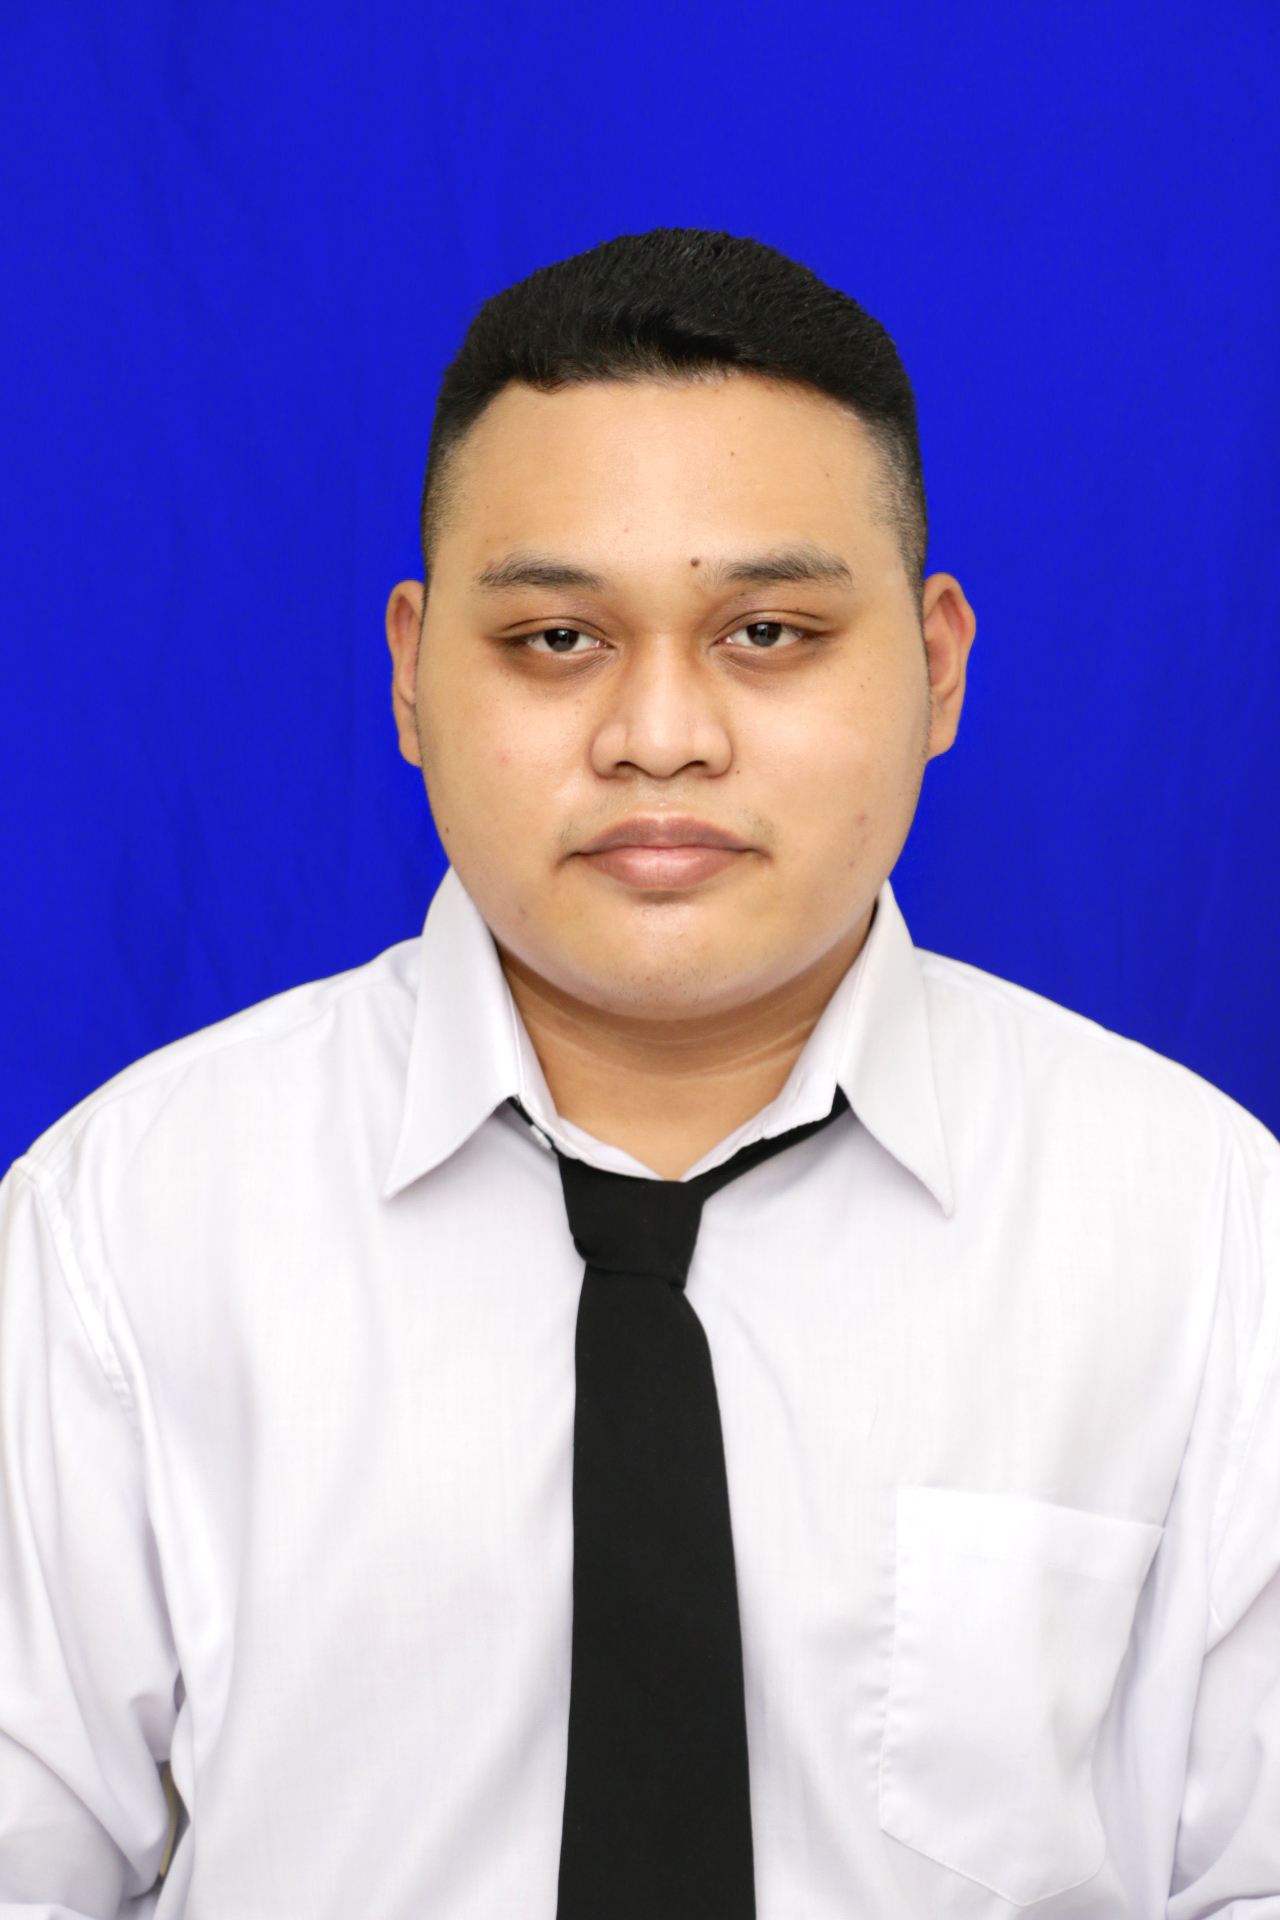
\includegraphics[width=.30\textwidth]{./gambar/Pas Foto Handar Ori.JPG}
    \vspace{-20pt} % Silahkan disesuaikan apabila space di bawah gambar terlalu kecil/besar
  \end{center}
\end{wrapfigure}

\noindent Nama lengkap penulis Hanandaru Mahaputra Purwanto, dengan nama panggilan Handar. Penulis dilahirkan di Surabaya, 23 September 2002, merupakan anak pertama dari dua bersaudara. Penulis telah menempuh pendidikan formal di SMPK Tegaljaya Badung dan SMAK Kolese Santo Yusup Malang. Setelah lulus dari SMA pada tahun 2021 penulis diterima di Departemen Fisika FSAD-ITS dan terdaftar sebagai mahasiswa dengan NRP 5001211007. Selama duduk di bangku kuliah penulis aktif mengikuti kegiatan perkuliahan. Di Departemen Fisika ITS, penulis mengambil bidang studi fisika material. Penulis pernah menjadi asisten laboratorium mata kuliah Fisika Mekanika dan Fisika Listrik dan Magnet. Penulis memiliki ketertarikan pada bidang simulasi sistem kuantum, fisika zat mampat, dan DFT.
 
\vspace{7pt}
\noindent Email: \emailMahasiswa

%======================================================================